\documentclass[tikz,border=2pt]{standalone}
\usetikzlibrary{calc}
\usepackage{bm}

\begin{document}

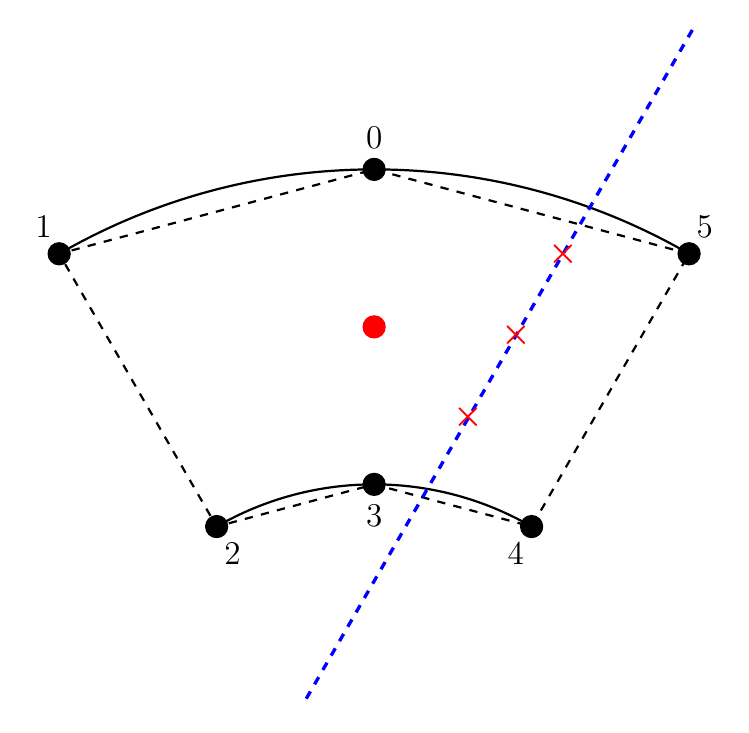
\begin{tikzpicture}[scale=4]
    % only show the relevant part
    % replace draw by clip
    \clip (-1.1, 0.3) rectangle (1.1, 2.45);
    
    %\node at (0,0) {$\times$};
    % outer layer
    \draw [thick] (0,0) ++(60:2cm) arc [start angle = 60, end angle = 120, radius = 2 cm];
    \filldraw[color=black] (60:2cm) circle [radius=1pt];
    \filldraw[color=black] (90:2cm) circle [radius=1pt];
    \filldraw[color=black] (120:2cm) circle [radius=1pt];
    % inner layer
    \draw [thick] (0,0) ++(60:1cm) arc [start angle = 60, end angle = 120, radius = 1 cm];
    \filldraw[color=black] (60:1cm) circle [radius=1pt];
    \filldraw[color=black] (90:1cm) circle [radius=1pt];
    \filldraw[color=black] (120:1cm) circle [radius=1pt];
    % draw center (the sense wires)
    \filldraw[color=red] (90:1.5cm) circle [radius=1pt];
    % draw lines to connect the edges
    \draw [black, thick, dashed] (60:2cm) -- (90:2cm) -- (120:2cm) -- (120:1cm) -- (90:1cm) -- (60:1cm) -- (60:2cm);
    % add wire numerotation
    \node at (90:2.1cm)  {\large 0};
    \node at (120:2.1cm) {\large 1};
    \node at (120:0.9cm) {\large 2};
    \node at (90:0.9cm)  {\large 3};
    \node at (60:0.9cm)  {\large 4};
    \node at (60:2.1cm)  {\large 5};
    % draw track
    \draw [very thick, dashed, blue] (-0.4,0) -- ++(60:3cm);
    \node [red] at ($(-0.4,0)+(60:2cm)$) {\large $\bm{\times}$};
    \node [red] at ($(-0.4,0)+(60:1.7cm)$) {\large $\bm{\times}$};
    \node [red] at ($(-0.4,0)+(60:1.4cm)$) {\large $\bm{\times}$};
\end{tikzpicture}


\end{document}